% rara: biber
% arara: xelatex: { synctex: yes }
\documentclass{scrartcl}

\usepackage{amsmath}
\usepackage{amssymb}

\usepackage{tikz}
\usetikzlibrary{calc,shapes,matrix,fit,calc}
\usepackage{pgfplots}
\usepgfplotslibrary{groupplots}
\pgfplotsset{compat=newest}
\usepackage{lscape}


\pgfplotscreateplotcyclelist{algs}{%
	lime!80!black,every mark/.append style={fill=lime},mark=square*\\%
	red,every mark/.append style={fill=red},mark=triangle*\\%
	teal,every mark/.append style={fill=teal!80},mark=pentagon*\\%
	black,mark=star\\%
	purple!30!blue,every mark/.append style={fill=purple!30!blue},mark=diamond*\\%
	orange!80!black,every mark/.append style={solid,fill=orange},mark=*\\%
	yellow!80!black,every mark/.append style={fill=yellow},mark=diamond*\\%
	pink!50!red,every mark/.append style={solid,fill=pink!80!red},mark=*\\%
	purple!80!blue,every mark/.append style={solid,fill=purple},mark=*\\%
}

\pgfplotscreateplotcyclelist{algsbar}{%
	lime!80!black,fill=lime\\%
	red,fill=red\\%
	teal,fill=teal!80\\%
	black,fill=black!80\\%
	purple!30!blue,fill=purple!30!blue\\%
	orange!80!black,fill=orange\\%
	cyan!80!black,fill=cyan\\%
	yellow!80!black,fill=yellow\\%
	pink!80!black,fill=pink\\%
}

\pgfplotsset{
	plotlabels/.style={
			xlabel={Dataset},
			%xlabel style ={yshift=-2cm},
			xtick={
					fib41,
					cere,
					e\_coli,
					influenza,
					para,
					einstein\_de,
					einstein\_en,
					coreutils,
					kernel,
					worldleaders,
				},
			xticklabel style={rotate=-90},%, xshift=0.5cm, yshift=4mm,
		},
	plotticks/.style ={
			symbolic x coords={
					fib41,
					cere,
					e\_coli,
					influenza,
					para,
					einstein\_de,
					einstein\_en,
					coreutils,
					kernel,
					worldleaders,
				},
		}
}

\usepackage{todonotes}
\usepackage{hyperref}
\usepackage{cleveref}

\usepackage{caption}
\usepackage{subcaption}
\usepackage{enumitem}


\newcommand{\lzend}{LZ-End}
\newcommand{\tikzmark}[1]{\tikz[overlay,remember picture] \node (#1) {};}

\usepackage{biblatex}
\addbibresource{Random Access.bib}




\title{Evaluation of Random Access Data Structures for Repetetive Data}
\author{Etienne Palanga}

\begin{document}
\maketitle

\begin{abstract}
	We evaluate several compressed string representations and compare their space consumption in RAM,
	as well as the time required to extract single characters, or substrings of different sizes.
	We also introduce a simple random access data structure based on straight-line grammars.
\end{abstract}

\section{Introduction}

As data volume increasing in almost any field and as such, handling data in compressed form is gaining importance.
The question arises whether text, especially repetetive ones, can be represented in a way which reduces their memory footprint, while still allowing efficient retrieval of the original data.

Approaches to this problem are already known in the literature \cite{belazzougui_block_2021,bille_random_2013,kreft_self-index_2011,nunes_grammar_2022}.
In this short evaluation, we will compare implementations of several compressed data structures.
In this evaluation one is based on context-free grammars, one by \citeauthor{kreft_self-index_2011} is based on the \lzend{} parsing \cite{kreft_self-index_2011}, and another by \citeauthor{belazzougui_block_2021} is based on block trees \cite{belazzougui_block_2021}.

We will evaluate the space requirements as well as query speed for each of the data structures on several repetetive datasets from the Pizza \& Chili Corpus \footnote{\url{http://pizzachili.dcc.uchile.cl/}}.

\section{Data Structures}

For a text $T[1..n] \in \Sigma^n$ with length $n \in \mathbb{N}$ over an alphabet $\Sigma$, we aim to store $T$ in as little space as possible while retaining the ability to access single characters or substrings from $T$.
Various data structures exist to facilitate this.

\subsection{\lzend{}}

One data structure is \citeauthor{kreft_self-index_2011}'s \lzend{}-based data structure.
\lzend{} is a variation of the LZ77 parsing \cite{ziv_universal_1977} in which $T$ is split into phrases $T_f = f_1 f_2 \dots f_k$.
Each phrase $f_i$ is either a single character $c \in \Sigma$ or a pointer to the left in $T$ from which a previously occurring substring is copied. The additional restriction for \lzend{} is that the copied substring must be a suffix of $f_1 \dots f_j$ where $j < i$.
The single character following this copied substring is also part of $f_i$.
An example parsing is given in \cref{fig:02:lzend}, but formal definitions and the specific description of the data structure should be taken from the original paper \cite{kreft_self-index_2011}.
For this evaluation, the parsing is created by \citeauthor{kempa_lz-end_2017}'s implementation \cite{kempa_lz-end_2017}\footnote{\url{https://github.com/dominikkempa/lz-end-toolkit}}.
The random access data structure is generated from this parsing.

\subsection{Block Tree}

The next data structure is the block tree introduced by \citeauthor{belazzougui_block_2021} \cite{belazzougui_block_2021}.
As the name implies, it is a tree-like data structure.
For some parameters $s, \tau \geq 2$, we divide $T$ into $s$ blocks of equal size, then recursively divide the blocks into $\tau$ blocks of equal size.
This procedure is recursively applied to each block, yielding a $\tau$-ary tree, except for the root which has degree $s$.
This tree compressed by identifying blocks, whose content appears to the left of this block on the same level.
Such blocks are replaced by blocks pointing at the previous occurrence.
Again, for formal definitions and explanations of the data structure, we refer to the original paper by \citeauthor{belazzougui_block_2021} \cite{belazzougui_block_2021}.
In this evaluation, an implementation by Reyes\footnote{\url{https://github.com/elarielcl/MinimalistBlockTrees}} is used, which we augmented with support for faster substring operations.\footnote{\url{https://github.com/Skadic/MinimalistBlockTrees}}

\begin{figure}
	\centering
	\begin{equation}
		T_f = b|\tikzmark{anS}a|n|\tikzmark{an}\textcolor{red}{an}a|c|\tikzmark{ana}\textcolor{red}{ana}d|a
	\end{equation}

	\begin{tikzpicture}[overlay, remember picture]
		\begin{scope}[transform canvas={xshift=0.75mm}]
			\draw[->,shorten >=5pt,shorten <=5pt,out=-90,in=-90,distance=0.5cm] (an.north) to (anS.north);
		\end{scope}
		\begin{scope}[transform canvas={xshift=1.25mm}]
			\draw[->,shorten >=5pt,shorten <=5pt,out=-90,in=-90,distance=0.5cm] (ana.north) to (an.north);
		\end{scope}
	\end{tikzpicture}

	\caption{An example of an \lzend{} parsing for $T = bananacanada$. The parts copied from other parts of $T$ are marked in red and their sources are denoted by arrows.}
	\label{fig:02:lzend}
\end{figure}

\subsection{Sampled Scan Grammar}

This is a simple data structure based for strings compressed as straight-line grammars, borrowing definitions from \citeauthor{benz_effective_2013}'s paper \cite{benz_effective_2013}.

\paragraph{Straight-Line Grammars} A \emph{context-free grammar} $G = (\mathcal{N}, \Sigma, P, S)$ is comprised of \emph{non-terminals} $\mathcal{N}$,
\emph{terminals} $\Sigma$ with $\mathcal{N} \cap \Sigma = \emptyset$,
\emph{production rules} $P$ where each rule is of the form $(X \rightarrow \alpha) \in P$ with $X \in \mathcal{N}, \alpha \in (\mathcal{N} \cup \Sigma)^*$.
$X$ is called the \emph{left side} of the rule and $\alpha$ the \emph{right side}.
Lastly, there is a designated \emph{start symbol} $S \in \mathcal{N}$

The expansion $\overset{*}{\rightarrow}$ of a string $(\mathcal{N} \cup \Sigma)^*$ results
by iteratively replacing each non-terminal with a corresponding right side of a rule in $P$
until only terminals remain.
Then we call $L(G) = \{ \alpha\ |\ S \overset{*}{\rightarrow} \alpha \}$, which is the set of all expansions of $S$, the \emph{language} of $G$.

A \emph{straight-line grammar} is a special case of a context-free grammar, where $|L(G)| = 1$.
That is, the grammar only produces one single string. In particular, this also means that the expansion of every non-terminal $X \in \mathcal{N}$ is unique and will be denoted by $ex(X)$.

\paragraph{Sampling} The idea of this data structure is to regularly sample positions in the text and locate them in the grammar, then to save those sample positions.
We sample the positions in such a way, that each sampled position guarantees that we can reach the entirety of the surrounding block from that sample.
When a query is made, we jump to a close sampled position and scan through the grammar for the rest of the way.

Let $T[1..n] \in \Sigma^n$ be a string and $G_T = (\mathcal{N}, \Sigma, P, S)$ a straight-line grammar that produces $T$.
The \emph{sampled scan} data structure saves the number of symbols in each production rule's right side.
For some parameter $r \in \mathbb{N}$ and $r < n$ called the \emph{sampling rate}, we divide $T$ into blocks $T = b_1 \dots b_k$ each of size $r$.

For each block $b_k$, we search for the rule $(X \rightarrow \alpha) \in P$ where $|ex(X)|$ is minimal and $ex(X)$ covers $b_k$ entirely.
We then choose the left-most symbol $c \in \mathcal{N} \cup \Sigma$ in $\alpha$ where $ex(c)$ \emph{starts} inside of $b_k$.
Let $p_\alpha$ be the position of $c$ in $\alpha$ and $p_{b_k}$ the start position of $ex(c)$ in $b_k$. We save the location of $c$ by storing the tuple $s_k := (X, i_\alpha, p_{b_k})$

\subparagraph{Example}

An example is depicted in \cref{fig:02:samplingexample}.
A straight-line grammar for $T = ababacaababa$ and a sampling rate of $r=3$.
and a visual representation are given in \cref{subfig:02:grammar,subfig:02:grammarvisual} respectively.
The sampled symbols are marked in purple.

To calculate the sample for $b_4 = T[10..12]$, we choose the rule that covers it entirely and has a minimally small expansion.
In this case, this is the second $A$. Now we choose the first symbol in that $A$ whose expansion starts in the block $T[10..12]$.
This is the second $B$ in the right side of $A$  at index $3$. Its expansion starts at index $11$ in $T$ which corresponds to index $2$ inside of $T[10..12]$.
This results in the sample: $s_4 = (A, 3, 2)$;

In total we end up with these samples: $(A, 1, 1), (S, 2, 3), (S, 3, 1), (A, 3, 2)$.

\begin{figure}
	\centering
	\begin{subfigure}{0.4\textwidth}
		\centering
		\begin{align*}
			S                   & \rightarrow AcaA \\
			\textcolor{cyan}{A} & \rightarrow aBB  \\
			\textcolor{red}{B}  & \rightarrow ba
		\end{align*}
		\caption{A straight-line grammar for $T$.}
		\label{subfig:02:grammar}
	\end{subfigure}
	\hfill
	\begin{subfigure}{0.5\textwidth}
		\centering
		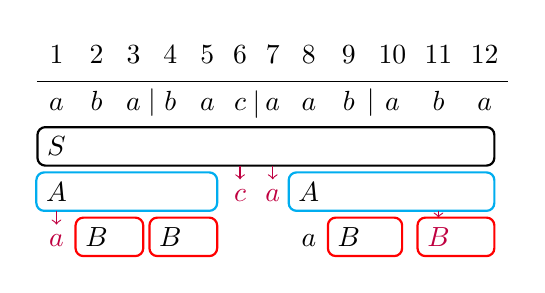
\begin{tikzpicture}
			\node[matrix of nodes, column sep=0mm, row sep=1mm, nodes in empty cells] (m) {
				$1$ & $2$ & $3$ & $4$ & $5$ & $6$ & $7$ & $8$ & $9$ & $10$ & $11$ & $12$\\\hline
				$a$ & $b$ & $a$ & $b$ & $a$ & $c$ & $a$ & $a$ & $b$ & $a$ & $b$ & $a$\\
				$S$ & & & & & & & & & & & \\
				$A$ & & & & & \textcolor{purple}{$c$} & \textcolor{purple}{$a$} & $A$ & & & & \\
				\textcolor{purple}{$a$} & $B$ & & $B$ & & & & $a$ & $B$ & & \textcolor{purple}{$B$} & \\
			};

			% Separators
			\node at ($(m-2-3)!0.5!(m-2-4)$) {$|$};
			\node at ($(m-2-6)!0.5!(m-2-7)$) {$|$};
			\node at ($(m-2-9)!0.5!(m-2-10)$) {$|$};

			\node[fit={(m-3-1.north west) (m-3-12.south east)},
				thick, inner sep=0, rounded corners=1mm,
				draw=black]{};

			\node[fit={(m-4-1.north west) (m-4-5.south east)},
				thick, inner sep=0, rounded corners=1mm,
				draw=cyan]{};
			\node[fit={(m-4-8.north west) (m-4-12.south east)},
				thick, inner sep=0, rounded corners=1mm,
				draw=cyan]{};

			\node[fit={(m-5-2.north west) (m-5-3.south east)},
				thick, inner sep=0, rounded corners=1mm,
				draw=red]{};
			\node[fit={(m-5-4.north west) (m-5-5.south east)},
				thick, inner sep=0, rounded corners=1mm,
				draw=red]{};
			\node[fit={(m-5-9.north west) (m-5-10.south east)},
				thick, inner sep=0, rounded corners=1mm,
				draw=red]{};
			\node[fit={(m-5-11.north west) (m-5-12.south east)},
				thick, inner sep=0, rounded corners=1mm,
				draw=red]{};

			\draw[->,purple] (m-4-1) -- (m-5-1);
			\draw[->,purple] (m-3-6) -- (m-4-6);
			\draw[->,purple] (m-3-7) -- (m-4-7);
			\draw[->,purple] (m-4-11) -- (m-5-11);
		\end{tikzpicture}
		\caption{Visual representation of the grammar.}
		\label{subfig:02:grammarvisual}
	\end{subfigure}
	\caption{An example of sampling with a grammar for the string $T = ababacaababa$. The chosen sampling rate is $r=3$.}
	\label{fig:02:samplingexample}
\end{figure}

\subsubsection{Queries}

Random access and substring queries follow the same general principle.
We choose the sample that lies in the same block as the query index.
From there, we scan until we have found the character or extracted all characters of the substring.

\paragraph{Random Access}

To answer a random access query for $1 \leq i \leq n$, we first determine the block $i$ is contained in, that being $k := \lceil i/r \rceil$.
Let $s_k =: (X, p_{\alpha}, p_{b_k}) \in (\mathcal{N} \cup \Sigma) \times \mathbb{N} \times \mathbb{N}$, where $\alpha$ is the right side of $X$.
Then we know that $\alpha$ contains the character we are looking for since it spans the entire block $b_k$.
Depending on whether $i$ is lesser or greater than $k \cdot r + p_{b_k}$, we now just need to scan either backwards or forwards respectively,
descending into other nonterminals if necessary, in order to find the desired character.
While scanning we skip nonterminals that do not contain $i$ by making use of the saved length of the nonterminals' right side.

\paragraph{Substring}

Answering a substring query for $T[i..j]$ is similar to the random access query.
However, we answer a substring query block-wise. For each block that $T[i..j]$ spans we have a separate query.

For each of these queries we again find the correct sample $s_k$.
We then scan for the positions $i$ and $j$ and while doing so, instead of skipping non-terminals that do not contain $i$ and $j$
we return each terminal we encounter that is in $T[i..j]$.
This of course might require a forward \emph{and} backwards scan each block.

\section{Evaluation}

In this evaluation we will be comparing the aforementioned data structures and compare their performance and space usage with \texttt{std::string} from the C++ standard library.
The substring queries for \texttt{std::string} do not use the \texttt{substr} method.
Rather, we use the \texttt{std::copy} function to copy the characters into a preallocated \texttt{char} buffer.
Similarly, the queries on the other data structures also copy characters into a preallocated buffer.

The experiments were conducted on a machine running Ubuntu 18.04 with two AMD EPYC 7452 Processors with 32 physical cores (64 logical cores) each running at 2.35GHz base clock rate.

\subsection{Datasets}

All datasets used in this evaluation stem from the Pizza \& Chili repetetive Corpus \footnote{\url{http://pizzachili.dcc.uchile.cl/}}.
Among them are  artificial and real texts.

\paragraph{Artificial}

These are texts that are calculated from a mathematical definition and do not stem from a real-life source.

\begin{itemize}[leftmargin=2cm]
	\item[\textbf{fib41}] If $S_0 = 0$ and $S_1 = 01$ then $S_n = S_{n-1}S_{n-2}$,
		then the concatenation of the previous two words, is called the $n$-th \emph{Fibonacci word}. \cite{barabash_periodic_2016}
		This is $S_{41}$.
\end{itemize}

\paragraph{Real}

These are texts that come from real-live sources and are \emph{not} artificially made repetetive.

\begin{itemize}[leftmargin=2cm]
	\item[\textbf{cere}] $37$ sequences of the yeast \emph{Saccharomyces Cerevisiae}'s genome.
	\item[\textbf{e\_coli}] $23$ sequences of the bacterium \emph{Escherichia Coli}'s genome.
	\item[\textbf{influenza}] $78,041$ sequences of the bacterium \emph{Haemophilus Influenzae}'s genome.
	\item[\textbf{para}] $32$ sequences of the yeast \emph{Saccharomyces Paradoxus}'s genome.
	\item[\textbf{einstein}] All versions of the Albert Einstein Wikipedia article in English and German respectively.
	\item[\textbf{coreutils}] The source code of all 5.x versions of the GNU Coreutils package totalling in 9 versions.
	\item[\textbf{kernel}] The source code of all 1.0.x and 1.1.x versions of the Linux kernel totalling in 36 versions.
	\item[\textbf{worldleaders}] The pdf files of CIA World Leaders from January 2003 to December 2009, converted to text.
\end{itemize}

Statistics concerning each dataset can be found in \cref{tab:03:datastats}.

\begin{table}
	\caption{Statistics for all used datasets.}
	\label{tab:03:datastats}
	\centering
	\begin{tabular}[c]{r|c|c}
		\textbf{Dataset}      & \textbf{Size (MiB)} & \textbf{Alphabet Size} \\\hline\hline
		\textbf{cere}         & $440$               & 5                      \\
		\textbf{e\_coli}      & $108$               & 15                     \\
		\textbf{influenza}    & $148$               & 15                     \\
		\textbf{para}         & $410$               & 5                      \\
		\textbf{einstein\_de} & $89$                & 117                    \\
		\textbf{einstein\_en} & $446$               & 139                    \\
		\textbf{coreutils}    & $196$               & 236                    \\
		\textbf{kernel}       & $247$               & 160                    \\
		\textbf{worldleaders} & $45$                & 89                     \\
	\end{tabular}
\end{table}

\subsection{Data Structures}

The data structures in use are the aforementioned ones.

For block trees, the relevant parameters are the arity $a \in \mathbb{N}$ of each block and the prefix/suffix size $ps \in \mathbb{N}_0$.
The prefix/suffix size (PS in the figure) is the number $ps$ such that each block in the tree saves its first and last $ps$ characters each, to facilitate faster substring queries.
If no data is saved ($ps = 0$) then the substring query is implemented naively, using random access queries for each character.
Other parameters have not shown to have a noticable effect, so they are omitted.
For the exact workings of the queries, we refer to the original paper by \citeauthor{belazzougui_block_2021} \cite{belazzougui_block_2021}.
In the figures, a block tree with arity $2$ and prefix suffix size $4$ would be labeled as A2PS4 for brevity's sake.

For sampled scan we use a sample parameter of $512$.
For every dataset we use a grammar created by Re-Pair \cite{larsson_off-line_2000} and Sequitur \cite{nevill-manning_identifying_1997} respectively.

There will be plots containing data for every data structure, however the block tree data will not contain all tested parameterizations, since this would clutter the graph.
In the general plots, there will be data for the best-compressing block tree parameterization (A2PS0) and the best-performing (A32PS16).
We will have additional plots containing only block tree data for this reason.

% IMPORT-DATA data benches.txt

\subsection{Query Speed}

Random Access (1 character) and substring queries were evaluated.
Each query was run $10^6$ times, and substring queries of lengths $10$, $100$, $1,000$ and $10,000$ were performed.
Though, for substrings, only figures for lengths $10$ and $10,000$ will be showcased here.

\subsubsection{Random Access}

Out of the compressed formats, the block tree is the clear winner in most cases, the A32PS16 parameterization never being slower than $\texttt{std::string}$ by a factor of more than $4$,
most of the time being ahead by several orders of magnitude in comparison to the others.
We can see that the block tree's arity does have a performance impact, with higher arity block trees performing better than lower arity block trees.
We also see that for sampled scan, whether the datastructure built on the RePair or Sequitur grammar is faster depends on the dataset.
But all in all the difference is not significant and the grammars were in many cases several orders of magnitude slower than the block trees.
The \lzend{} data structure was the slowest on every dataset in this benchmark.

\begin{figure}[t]
	\begin{tikzpicture}
		\begin{groupplot}[height=25cm,group style={group size= 1 by 2}]
			\nextgroupplot[
				title={Random Access},
				width=15cm,
				height=8cm,
				ylabel={Time for $10^{6}$ queries [$\lg_{2}$ ms]},
				legend pos=north east,
				plotticks,
				plotlabels,
				ybar,
				bar width=1.2mm,
				cycle list name=algsbar,
        legend style={at={(0.5,1.25)},anchor=center},
        legend columns=3
			]
			%% MULTIPLOT(ds,filetype,arity) SELECT input_file AS x, MIN(LOG(2, query_time_total)) AS y, MULTIPLOT
			%% FROM data WHERE type='random_access' AND NOT input_file LIKE "%200"
			%% GROUP BY filetype, input_file, MULTIPLOT ORDER BY MULTIPLOT,x
   \addplot coordinates { (cere,8.02237) (coreutils,8.17991) (e\_coli,7.88264) (einstein\_de,8.02791) (einstein\_en,8.25739) (fib41,8.29921) (influenza,7.62936) (kernel,8.15987) (para,8.0) (worldleaders,7.89482) };
   \addlegendentry{A2PS*};
   \addplot coordinates { (cere,7.03342) (coreutils,7.11894) (e\_coli,6.75489) (einstein\_de,6.22882) (einstein\_en,6.56986) (fib41,6.83289) (influenza,6.53916) (kernel,6.80735) (para,6.9542) (worldleaders,6.08746) };
   \addlegendentry{A32PS*};
   \addplot coordinates { (cere,12.9549) (coreutils,13.3012) (e\_coli,12.7634) (einstein\_de,12.4686) (einstein\_en,12.9121) (fib41,13.4246) (influenza,13.2559) (kernel,12.8803) (para,12.9706) (worldleaders,13.67) };
   \addlegendentry{LzEnd};
   \addplot coordinates { (cere,10.774) (coreutils,10.7814) (e\_coli,10.668) (einstein\_de,8.88264) (einstein\_en,8.93958) (fib41,7.47573) (influenza,9.90539) (kernel,10.8865) (para,10.8634) (worldleaders,8.96867) };
   \addlegendentry{Sampled Scan (RePair)};
   \addplot coordinates { (cere,10.733) (coreutils,10.5255) (e\_coli,9.89482) (einstein\_de,8.60733) (einstein\_en,8.99435) (fib41,7.47573) (influenza,10.5333) (kernel,10.6519) (para,10.6537) (worldleaders,9.3837) };
   \addlegendentry{Sampled Scan (Sequitur)};
   \addplot coordinates { (cere,5.32193) (coreutils,5.2854) (e\_coli,5.20945) (einstein\_de,5.20945) (einstein\_en,5.32193) (fib41,5.24793) (influenza,5.2854) (kernel,5.32193) (para,5.32193) (worldleaders,5.08746) };
   \addlegendentry{\texttt{std::string}};
		\end{groupplot}
	\end{tikzpicture}
	\caption{Random access query speed for $10^6$ queries.}
	\label{fig:03:raspeed}
\end{figure}

\subsubsection{Substring}

As depicted in \cref{fig:03:ssspeed}, with substring queries the A32PS16 block tree still beats sampled scan.
On very short substrings the block tree is several orders of magnitude faster than the grammar in most cases.
The exception here is \textbf{fib41} at which the grammar is only slower by a factor of about $2$.
This only applies to the A32PS16 parameterization though, as the A2PS0 block tree is now the slowest data structure on long substrings.

On substrings of length $10,000$ this advantage shrinks significantly.
While the A32PS16 block tree is on average around a factor of $4$ faster than the grammar,
it is still much slower than \texttt{std::string}.
This is usually by a factor of around $2^6$ while the grammar hovers around being approximately $2^8$
times slower than \texttt{std::string}.

Even though the A2PS0 tree was the slowest block tree it still beat the \lzend{} data structure on every dataset except for \textbf{fib41},
usually being about $4-8$ times faster.


\begin{figure}
	\begin{tikzpicture}
		\begin{groupplot}[height=25cm,group style={group size= 1 by 2}]
			\nextgroupplot[
				title={Substrings of length $10$},
				width=15cm,
				height=8cm,
				ylabel={Time for $10^{6}$ queries [$\lg_{2}$ ms]},
				legend pos=north east,
				plotticks,
				xtick=\empty,
				ybar,
				bar width=1.2mm,
				cycle list name=algsbar,
        legend style={at={(0.5,1.25)},anchor=center},
        legend columns=3
			]
			%% MULTIPLOT(ds,filetype,arity,prefix_suffix) SELECT input_file AS x, MIN(LOG(2, query_time_total)) AS y, MULTIPLOT
			%% FROM data
			%% WHERE type='substring' AND NOT input_file LIKE "%200" AND substring_length=10 
			%% AND (arity=2 AND prefix_suffix=0 OR arity=32 AND prefix_suffix=16 or ds!='blocktree')  
			%% GROUP BY filetype, input_file, MULTIPLOT ORDER BY MULTIPLOT,x
   \addplot coordinates { (cere,10.8065) (coreutils,11.0478) (e\_coli,10.7731) (einstein\_de,10.9887) (einstein\_en,11.1261) (fib41,11.3443) (influenza,10.3783) (kernel,11.0967) (para,10.7245) (worldleaders,10.9144) };
   \addlegendentry{A2PS0};
   \addplot coordinates { (cere,7.5157) (coreutils,7.65105) (e\_coli,7.31288) (einstein\_de,6.97728) (einstein\_en,7.16993) (fib41,7.32193) (influenza,7.26679) (kernel,7.37504) (para,7.45121) (worldleaders,6.93074) };
   \addlegendentry{A32PS16};
   \addplot coordinates { (cere,14.9031) (coreutils,15.0466) (e\_coli,14.6792) (einstein\_de,14.059) (einstein\_en,14.2167) (fib41,14.1718) (influenza,14.7515) (kernel,14.855) (para,14.7967) (worldleaders,15.0138) };
   \addlegendentry{LzEnd};
   \addplot coordinates { (cere,11.0841) (coreutils,11.1799) (e\_coli,11.0133) (einstein\_de,9.5411) (einstein\_en,9.66) (fib41,8.33539) (influenza,10.3151) (kernel,11.2432) (para,11.1674) (worldleaders,9.59991) };
   \addlegendentry{Sampled Scan (RePair)};
   \addplot coordinates { (cere,11.1046) (coreutils,11.1222) (e\_coli,10.4988) (einstein\_de,9.41574) (einstein\_en,9.70908) (fib41,8.37938) (influenza,11.0007) (kernel,11.1755) (para,11.032) (worldleaders,10.021) };
   \addlegendentry{Sampled Scan (Sequitur)};
   \addplot coordinates { (cere,5.75489) (coreutils,5.72792) (e\_coli,5.64386) (einstein\_de,5.64386) (einstein\_en,5.75489) (fib41,5.70044) (influenza,5.70044) (kernel,5.72792) (para,5.72792) (worldleaders,5.52356) };
   \addlegendentry{\texttt{std::string}};

			\nextgroupplot[
				title={Substrings of length $10,000$},
				width=15cm,
				height=8cm,
				ylabel={Time for $10^{6}$ queries [$\lg_{2}$ ms]},
				legend pos=north east,
				plotticks,
				plotlabels,
				ybar,
				bar width=1.2mm,
				cycle list name=algsbar
			]
			%% MULTIPLOT(ds,filetype,arity,prefix_suffix) SELECT input_file AS x, MIN(LOG(2, query_time_total)) AS y, MULTIPLOT
			%% FROM data WHERE type='substring' AND NOT input_file LIKE "%200" AND substring_length=10000
			%% AND (arity=2 AND prefix_suffix=0 OR arity=32 AND prefix_suffix=16 or ds!='blocktree')  
			%% GROUP BY filetype, input_file, MULTIPLOT ORDER BY MULTIPLOT,x
   \addplot coordinates { (cere,20.5576) (coreutils,20.842) (e\_coli,20.6036) (einstein\_de,20.6817) (einstein\_en,20.8775) (fib41,21.184) (influenza,20.1066) (kernel,20.8779) (para,20.4493) (worldleaders,20.6971) };
   \addplot coordinates { (cere,15.7818) (coreutils,15.8922) (e\_coli,15.5731) (einstein\_de,15.8991) (einstein\_en,16.0114) (fib41,16.3549) (influenza,15.3876) (kernel,15.9757) (para,15.773) (worldleaders,15.7193) };
   \addplot coordinates { (cere,24.1556) (coreutils,24.1378) (e\_coli,23.9044) (einstein\_de,23.108) (einstein\_en,22.9621) (fib41,20.1354) (influenza,23.6527) (kernel,24.1372) (para,23.9779) (worldleaders,23.6986) };
   \addplot coordinates { (cere,18.2669) (coreutils,18.307) (e\_coli,18.3196) (einstein\_de,17.8303) (einstein\_en,17.8559) (fib41,16.836) (influenza,17.8795) (kernel,18.2382) (para,18.4188) (worldleaders,17.5317) };
   \addplot coordinates { (cere,18.419) (coreutils,18.7239) (e\_coli,18.3401) (einstein\_de,17.793) (einstein\_en,17.9275) (fib41,16.8349) (influenza,18.5641) (kernel,18.628) (para,18.3881) (worldleaders,17.7543) };
   \addplot coordinates { (cere,9.93369) (coreutils,9.83763) (e\_coli,9.75322) (einstein\_de,9.72622) (einstein\_en,9.90689) (fib41,9.87191) (influenza,9.80574) (kernel,9.86264) (para,9.93221) (worldleaders,9.49386) };

		\end{groupplot}
	\end{tikzpicture}
	\caption{Substring query speed for $10^6$ queries.}
	\label{fig:03:ssspeed}
\end{figure}

In \cref{fig:03:ssspeedbt} results for the different parameterizations of block trees are depicted.

We can see that, the more data is saved in the prefixes and suffixes in each block, the faster the substring query becomes.
This is expected, as more saved characters allow for querying larger segments of the query at a time.
The decrease in runtime is fairly significant, as even just saving $4$ characters of each block's prefix and suffix leads to a speed up of at least factor $2$ on each dataset.
We also see that higher arity also decreases the run time.
This most likely follows from the fact, that each query need to traverse less levels of the tree.

While on substrings of length $10$, the fastest parameterization (A32PS16) was only slower by around a factor of $4$ on average
it was still around $2^6$ times slower than \texttt{std::string} for substring of length $10,000$.

\begin{figure}
	\begin{tikzpicture}
		\begin{groupplot}[height=25cm,group style={group size= 1 by 2}]
			\nextgroupplot[
				title={Substrings of length $10$ (Block Tree)},
				width=16cm,
				height=8cm,
				ylabel={Time for $10^{6}$ queries [$\lg_{2}$ ms]},
				legend pos=north east,
				plotticks,
				xtick=\empty,
				ybar,
				bar width=1mm,
				cycle list name=algsbar,
        legend style={at={(0.5,1.25)},anchor=center},
        legend columns=4
			]
			%% MULTIPLOT(ds,arity,prefix_suffix) SELECT input_file AS x, MIN(LOG(2, query_time_total)) AS y, MULTIPLOT
			%% FROM data WHERE type='substring' AND NOT input_file LIKE "%200" AND substring_length=10 AND (ds='blocktree' or ds='string')
			%% GROUP BY filetype, input_file, MULTIPLOT ORDER BY MULTIPLOT,x
   \addplot coordinates { (cere,10.8065) (coreutils,11.0478) (e\_coli,10.7731) (einstein\_de,10.9887) (einstein\_en,11.1261) (fib41,11.3443) (influenza,10.3783) (kernel,11.0967) (para,10.7245) (worldleaders,10.9144) };
   \addlegendentry{A2PS0};
   \addplot coordinates { (cere,9.52552) (coreutils,9.75822) (e\_coli,9.43254) (einstein\_de,9.62388) (einstein\_en,9.80574) (fib41,9.98726) (influenza,9.14211) (kernel,9.76818) (para,9.48784) (worldleaders,9.49586) };
   \addlegendentry{A2PS4};
   \addplot coordinates { (cere,8.33985) (coreutils,8.48784) (e\_coli,8.21917) (einstein\_de,8.18488) (einstein\_en,8.35755) (fib41,8.47168) (influenza,7.92481) (kernel,8.46352) (para,8.29462) (worldleaders,8.0607) };
   \addlegendentry{A2PS16};
   \addplot coordinates { (cere,8.8009) (coreutils,9.16491) (e\_coli,8.58496) (einstein\_de,8.85798) (einstein\_en,9.18488) (fib41,9.74483) (influenza,8.20945) (kernel,9.18735) (para,8.76155) (worldleaders,8.55842) };
   \addlegendentry{A32PS0};
   \addplot coordinates { (cere,7.97728) (coreutils,8.20945) (e\_coli,7.74819) (einstein\_de,7.75489) (einstein\_en,7.99435) (fib41,8.56605) (influenza,7.56224) (kernel,8.11894) (para,7.91886) (worldleaders,7.53916) };
   \addlegendentry{A32PS4};
   \addplot coordinates { (cere,7.5157) (coreutils,7.65105) (e\_coli,7.31288) (einstein\_de,6.97728) (einstein\_en,7.16993) (fib41,7.32193) (influenza,7.26679) (kernel,7.37504) (para,7.45121) (worldleaders,6.93074) };
   \addlegendentry{A32PS16};
   \addplot coordinates { (cere,5.75489) (coreutils,5.72792) (e\_coli,5.64386) (einstein\_de,5.64386) (einstein\_en,5.75489) (fib41,5.70044) (influenza,5.70044) (kernel,5.72792) (para,5.72792) (worldleaders,5.52356) };
   \addlegendentry{\texttt{std::string}};

			\nextgroupplot[
				title={Substrings of length $10,000$ (Block Tree)},
				width=16cm,
				height=8cm,
				ylabel={Time for $10^{6}$ queries [$\lg_{2}$ ms]},
				legend pos=north east,
				plotticks,
				plotlabels,
				ybar,
				bar width=1mm,
				cycle list name=algsbar
			]
			%% MULTIPLOT(ds,arity,prefix_suffix) SELECT input_file AS x, MIN(LOG(2, query_time_total)) AS y, MULTIPLOT
			%% FROM data WHERE type='substring' AND NOT input_file LIKE "%200" AND substring_length=10000 AND (ds='blocktree' or ds='string')
			%% GROUP BY filetype, input_file, MULTIPLOT ORDER BY MULTIPLOT,x
   \addplot coordinates { (cere,20.5576) (coreutils,20.842) (e\_coli,20.6036) (einstein\_de,20.6817) (einstein\_en,20.8775) (fib41,21.184) (influenza,20.1066) (kernel,20.8779) (para,20.4493) (worldleaders,20.6971) };
   \addplot coordinates { (cere,18.7889) (coreutils,19.042) (e\_coli,18.781) (einstein\_de,18.9752) (einstein\_en,19.1078) (fib41,19.4413) (influenza,18.3955) (kernel,19.0788) (para,18.6952) (worldleaders,18.9423) };
   \addplot coordinates { (cere,17.1533) (coreutils,17.294) (e\_coli,17.0865) (einstein\_de,17.2558) (einstein\_en,17.3386) (fib41,17.6095) (influenza,16.8191) (kernel,17.3217) (para,17.0529) (worldleaders,17.2465) };
   \addplot coordinates { (cere,18.3728) (coreutils,18.7968) (e\_coli,18.1782) (einstein\_de,18.6536) (einstein\_en,18.9981) (fib41,19.5404) (influenza,17.6393) (kernel,18.9274) (para,18.3572) (worldleaders,18.3521) };
   \addplot coordinates { (cere,16.8732) (coreutils,17.1904) (e\_coli,16.6747) (einstein\_de,17.0707) (einstein\_en,17.3762) (fib41,17.8553) (influenza,16.2874) (kernel,17.3102) (para,16.8629) (worldleaders,16.8267) };
   \addplot coordinates { (cere,15.7818) (coreutils,15.8922) (e\_coli,15.5731) (einstein\_de,15.8991) (einstein\_en,16.0114) (fib41,16.3549) (influenza,15.3876) (kernel,15.9757) (para,15.773) (worldleaders,15.7193) };
   \addplot coordinates { (cere,9.93369) (coreutils,9.83763) (e\_coli,9.75322) (einstein\_de,9.72622) (einstein\_en,9.90689) (fib41,9.87191) (influenza,9.80574) (kernel,9.86264) (para,9.93221) (worldleaders,9.49386) };

		\end{groupplot}
	\end{tikzpicture}
	\caption{Block tree substring query speed for $10^6$ queries.}
	\label{fig:03:ssspeedbt}
\end{figure}


\subsection{Space}

\begin{figure}
	\begin{tikzpicture}
		\begin{groupplot}[height=25cm,group style={group size= 1 by 2}]
			\nextgroupplot[
				title={Storage Space},
				width=15cm,
				height=8cm,
				ylabel={Space [\% of input size]},
				legend pos=north east,
				plotticks,
				xtick=\empty,
				ybar,
				bar width=1.2mm,
				cycle list name=algsbar,
        legend style={at={(0.5,1.25)},anchor=center},
        legend columns=3
			]
			%% MULTIPLOT(ds,filetype,arity,prefix_suffix) SELECT input_file AS x, MIN(space * 100.0 / input_size) AS y, MULTIPLOT
			%% FROM data WHERE NOT input_file LIKE "%200" AND ds!="string"
			%% AND (arity=2 AND prefix_suffix=0 OR arity=32 AND prefix_suffix=16 or ds!='blocktree')  
			%% GROUP BY filetype, input_file, MULTIPLOT ORDER BY MULTIPLOT,x
   \addplot coordinates { (cere,2.64078) (coreutils,5.01461) (e\_coli,11.1591) (einstein\_de,0.30455) (einstein\_en,0.169289) (fib41,0.00182745) (influenza,4.32016) (kernel,2.0553) (para,3.77156) (worldleaders,3.02533) };
   \addlegendentry{A2PS0};
   \addplot coordinates { (cere,13.0709) (coreutils,28.8438) (e\_coli,33.0989) (einstein\_de,6.04444) (einstein\_en,3.63183) (fib41,0.00144524) (influenza,28.6874) (kernel,11.3736) (para,14.0303) (worldleaders,33.1738) };
   \addlegendentry{A32PS16};
   \addplot coordinates { (cere,3.44954) (coreutils,7.57514) (e\_coli,18.7515) (einstein\_de,0.588544) (einstein\_en,0.325256) (fib41,0.0725531) (influenza,8.48877) (kernel,3.10165) (para,5.36822) (worldleaders,4.67683) };
   \addlegendentry{LzEnd};
   \addplot coordinates { (cere,3.66247) (coreutils,4.78419) (e\_coli,6.80754) (einstein\_de,2.46492) (einstein\_en,2.39754) (fib41,2.3438) (influenza,3.07129) (kernel,3.47155) (para,3.87532) (worldleaders,3.44297) };
   \addlegendentry{Sampled Scan (RePair)};
   \addplot coordinates { (cere,3.34277) (coreutils,3.77539) (e\_coli,4.81625) (einstein\_de,2.45602) (einstein\_en,2.40394) (fib41,2.3438) (influenza,3.63565) (kernel,3.14076) (para,3.366) (worldleaders,3.42611) };
   \addlegendentry{Sampled Scan (Sequitur)};

			\nextgroupplot[
				title={Storage Space (Block Trees)},
				width=15cm,
				height=8cm,
				ylabel={Space [\% of input size]},
				legend pos=north east,
				plotticks,
				plotlabels,
				ybar,
				bar width=1mm,
				cycle list name=algsbar,
        legend columns=3
			]
			%% MULTIPLOT(ds,arity,prefix_suffix) SELECT input_file AS x, MIN(space * 100.0 / input_size) AS y, MULTIPLOT
			%% FROM data WHERE NOT input_file LIKE "%200" AND ds="blocktree"
			%% GROUP BY filetype, input_file, MULTIPLOT ORDER BY MULTIPLOT,x
   \addplot coordinates { (cere,2.64078) (coreutils,5.01461) (e\_coli,11.1591) (einstein\_de,0.30455) (einstein\_en,0.169289) (fib41,0.00182745) (influenza,4.32016) (kernel,2.0553) (para,3.77156) (worldleaders,3.02533) };
   \addlegendentry{A2PS0};
   \addplot coordinates { (cere,5.12006) (coreutils,17.2897) (e\_coli,24.1401) (einstein\_de,1.16203) (einstein\_en,0.696629) (fib41,0.00222758) (influenza,12.7618) (kernel,6.49618) (para,6.9103) (worldleaders,11.6888) };
   \addlegendentry{A2PS4};
   \addplot coordinates { (cere,12.3377) (coreutils,37.2673) (e\_coli,51.7463) (einstein\_de,3.14863) (einstein\_en,1.88739) (fib41,0.00248736) (influenza,32.3489) (kernel,12.9805) (para,16.0016) (worldleaders,29.9016) };
   \addlegendentry{A2PS16};
   \addplot coordinates { (cere,6.30836) (coreutils,17.8846) (e\_coli,22.4602) (einstein\_de,1.55953) (einstein\_en,0.854001) (fib41,0.000958515) (influenza,15.9965) (kernel,6.02301) (para,7.80101) (worldleaders,14.7503) };
   \addlegendentry{A32PS0};
   \addplot coordinates { (cere,7.99903) (coreutils,20.6245) (e\_coli,25.12) (einstein\_de,2.68259) (einstein\_en,1.58092) (fib41,0.00113171) (influenza,19.1693) (kernel,7.44751) (para,9.69558) (worldleaders,19.3564) };
   \addlegendentry{A32PS4};
   \addplot coordinates { (cere,13.0709) (coreutils,28.8438) (e\_coli,33.0989) (einstein\_de,6.04444) (einstein\_en,3.63183) (fib41,0.00144524) (influenza,28.6874) (kernel,11.3736) (para,14.0303) (worldleaders,33.1738) };
   \addlegendentry{A32PS16};
		\end{groupplot}
	\end{tikzpicture}
	\caption{Storage space in RAM for the compressed formats.}
	\label{fig:03:space}
\end{figure}

For space measurements, we observe in \cref{fig:03:space} that the results are mixed.
While the A2PS0 block tree consistently provides better compression than \lzend{}, they are matched closely or even beat by sampled scan.
The notable exceptions to this are \textbf{fib41} and the \textbf{einstein} datasets which show block trees and \lzend{} pulling ahead of the grammars significantly.
\textbf{fib41} is the more extreme case here, block trees requiring a mere $0.1\%$ space of its input, even on its A32PS16 parameterization.
The grammars on the other hand required around $2.34\%$ space.

We can also see that the size of \lzend{} correlates with the size of block trees.
While \lzend{} seems to have a larger overhead or worse compression overall, whenever \lzend{} compressed very efficiently (e.g. \textbf{fib41} or \textbf{einstein}),
block trees also do, taking up even less space.
The most likely reason for this that both of these data structures form an approximation of the LZ77 parsing \cite{ziv_universal_1977,belazzougui_block_2021,kempa_lz-end_2017}.

An interesting property of the block tree results is the relation of their arity and prefix/suffix size to their resulting size.
When looking at the block trees with arity $2$, we can see that even though it compresses better than arity $32$ at a base level,
increasing the prefix/suffix size leads to a dramatic increase in space consumption.
For example, on the \textbf{e\_coli} dataset, the arity $2$ block tree goes from $11\%$ at $ps = 0$ to $24\%$ at $ps=4$ to finally $51\%$ space at $ps=16$.
Almost a fivefold increase in space.
On the other hand, while the arity $32$ block tree starts out at a higher $22\%$ space, it only increases to $25\%$ and ends up at $33\%$, significantly lower than the arity $2$ block tree.
This is a trend that can be seen on most of the other datasets as well.

We can see, that if the objective is to support faster substring queries, it seems to be more beneficial to start out with a higher arity, even though that may lead to less compression initially.
Not only does the higher arity itself accelerate queries, but saving more prefix and suffix data seems to be much less costly than on low arity trees.

\section{Conclusion}

We have evaluated several compressed data structures in respect of their random access and substring queries and also their space consumption.
When it comes to query speed, \emph{block trees} show the highest query speed, beating all others on any dataset by various amounts.
On the other hand, if compression is the priority, then grammars show compression matching or beating block trees in many cases except on extremely repetetive data.
Block trees were only keeping up by not storing any prefix/suffix data (A2PS0) and while compressing well as seen in \cref{fig:03:ssspeedbt} have a very slow substring query speed.

In conclusion, if on repetetive data high compression is the most important objective and substring queries are of lower importance,
then block trees without any prefix/suffix data seem to offer the best trade-offs.
They compress reasonably well in most cases and also offer fast random access queries.

If substring queries are a priority then high-arity block trees with prefix/suffix data or grammars seem to be the best choice.
The block trees seem to compress a bit less efficiently in the majority of cases but offered higher performance.
Grammars on the other hand seemed to compress a bit more consistently and efficiently, while having worse performance.

\printbibliography


\end{document}
